\documentclass[
11pt, % The default document font size, options: 10pt, 11pt, 12pt
%codirector, % Uncomment to add a codirector to the title page
]{charter} 




% El títulos de la memoria, se usa en la carátula y se puede usar el cualquier lugar del documento con el comando \ttitle
\titulo{Monitoreo de consumo eléctrico en viviendas y departamentos} 

% Nombre del posgrado, se usa en la carátula y se puede usar el cualquier lugar del documento con el comando \degreename
%\posgrado{Carrera de Especialización en Sistemas Embebidos} 
\posgrado{Carrera de Especialización en Internet de las Cosas} 
%\posgrado{Carrera de Especialización en Intelegencia Artificial}
%\posgrado{Maestría en Sistemas Embebidos} 
%\posgrado{Maestría en Internet de las cosas}

% Tu nombre, se puede usar el cualquier lugar del documento con el comando \authorname
\autor{Ing. Cristian Matias Garcia} 

% El nombre del director y co-director, se puede usar el cualquier lugar del documento con el comando \supname y \cosupname y \pertesupname y \pertecosupname
\director{Mg. Ing. Martin Rodriguez}
\pertenenciaDirector{PSA} 
% FIXME:NO IMPLEMENTADO EL CODIRECTOR ni su pertenencia
%\codirector{Ariel Luthenberg} % para que aparezca en la portada se debe descomentar la opción codirector en el documentclass
%\pertenenciaCoDirector{FIUBA}

% Nombre del cliente, quien va a aprobar los resultados del proyecto, se puede usar con el comando \clientename y \empclientename
\cliente{Mg. Ing. Martin Rodriguez}
\empresaCliente{PSA}

% Nombre y pertenencia de los jurados, se pueden usar el cualquier lugar del documento con el comando \jurunoname, \jurdosname y \jurtresname y \perteunoname, \pertedosname y \pertetresname.
\juradoUno{Nombre y Apellido (1)}
\pertenenciaJurUno{pertenencia (1)} 
\juradoDos{Nombre y Apellido (2)}
\pertenenciaJurDos{pertenencia (2)}
\juradoTres{Nombre y Apellido (3)}
\pertenenciaJurTres{pertenencia (3)}
 
\fechaINICIO{17 de octubre de 2023}		%Fecha de inicio de la cursada de GdP \fechaInicioName
\fechaFINALPlan{5 de diciembre de 2023} 	%Fecha de final de cursada de GdP
\fechaFINALTrabajo{21 de agosto de 2024}	%Fecha de defensa pública del trabajo final


\begin{document}

\maketitle
\thispagestyle{empty}
\pagebreak


\thispagestyle{empty}
{\setlength{\parskip}{0pt}
\tableofcontents{}
}
\pagebreak


\section*{Registros de cambios}
\label{sec:registro}


\begin{table}[ht]
\label{tab:registro}
\centering
\begin{tabularx}{\linewidth}{@{}|c|X|c|@{}}
\hline
\rowcolor[HTML]{C0C0C0} 
Revisión & \multicolumn{1}{c|}{\cellcolor[HTML]{C0C0C0}Detalles de los cambios realizados} & Fecha      \\ \hline
 0      & Creación del documento                                 & 17/10/2023 \\ \hline
1.0      & Se completa hasta el punto 5 inclusive                & 31/10/2023 \\ \hline
2.0      & Se completa hasta el punto 9 inclusive, con correcciones de la version 1.0               & 07/11/2023 \\ \hline
%2      & Se completa hasta el punto 7 inclusive
%		  Se puede agregar algo más \newline
%		  En distintas líneas \newline
%		  Así                                                    & dd/mm/aaaa \\ \hline
%3      & Se completa hasta el punto 11 inclusive                & dd/mm/aaaa \\ \hline
%4      & Se completa el plan	                                 & dd/mm/aaaa \\ \hline
\end{tabularx}
\end{table}

\pagebreak



\section*{Acta de constitución del proyecto}
\label{sec:acta}

\begin{flushright}
Buenos Aires, \fechaInicioName
\end{flushright}

\vspace{2cm}

Por medio de la presente se acuerda con el Ing. \authorname\hspace{1px} que su Trabajo Final de la \degreename\hspace{1px} se titulará ``\ttitle'', consistirá esencialmente en la implementación de un sistema IoT aplicado al  control de consumo eléctrico en viviendas y/o departamentos, y tendrá un presupuesto preliminar estimado de 508 h de trabajo y \textcolor{red}{\$XXX}, con fecha de inicio \fechaInicioName\hspace{1px} y fecha de presentación pública \fechaFinalName.

Se adjunta a esta acta la planificación inicial.

\vfill

% Esta parte se construye sola con la información que hayan cargado en el preámbulo del documento y no debe modificarla
\begin{table}[ht]
\raggedleft
%\center
\begin{tabular}{ccc}
\begin{tabular}[c]{@{}c@{}} \supname \\ Director posgrado \end{tabular} \hspace{2cm} & %\begin{tabular}[c]{@{}c@{}}\clientename \\ \empclientename \end{tabular} 
\vspace{10.5cm} \\ 
%\hspace{2cm} \\ 
%\multicolumn{3}{c}{\begin{tabular}[c]{@{}c@{}} \supname \\ Director del Trabajo Final\end{tabular}} \vspace{2.5cm} \\
%\begin{tabular}[c]{@{}c@{}}\jurunoname \\ Jurado del Trabajo Final\end{tabular}     &  & \begin{tabular}[c]{@{}c@{}}\jurdosname\\ Jurado del Trabajo Final\end{tabular}  \vspace{2.5cm}  \\
%\multicolumn{3}{c}{\begin{tabular}[c]{@{}c@{}} \jurtresname\\ Jurado del Trabajo Final\end{tabular}} \vspace{.5cm}                                                                     
\end{tabular}
\end{table}






\section{1. Descripción técnica-conceptual del proyecto a realizar}
\label{sec:descripcion}


El presente proyecto es un emprendimiento personal que implementara un sistema de monitoreo de consumo eléctrico en viviendas y departamentos.
El proyecto  se desarrollara en el siguiente contexto:

\begin{itemize}

	\item{El consumo ineficiente de energía eléctrica en las viviendas de Argentina.
	}
	\item{La electricidad producida en las centrales eléctricas no permite cubrir la demanda eléctrica y provoca cortes en el suministro eléctrico de las viviendas. Debido a la demanda eléctrica las empresas imponen penalidades para los usuarios que superan ciertos umbrales de consumo eléctrico.
	}
	\item{El usuario solo puede verificar el consumo eléctrico con el resumen electrónico mensual y por inspección visual en el medidor de su domicilio.
	}
\end{itemize}


En esta situación se plantean los siguientes inconvenientes:

\begin{itemize}

	\item{No se puede determinar cuál es el promedio de cada electrodoméstico y evitar consumos innecesarios.
	}
	\item{Dos o más casas, dentro de un mismo domicilio, no pueden saber el consumo eléctrico correspondiente a cada una.
	}
	\item{En edificios con luz de obra no se puede saber el consumo de cada vivienda o  dividir el gasto del consumo eléctrico. Para los edificios se toma el total de consumo y se divide sobre el total de las viviendas.
	}
	\item{Se pierde el control del consumo eléctrico.
	}
	\item{Se produce el uso ineficiente de la energía eléctrica eléctrica.
	}
\end{itemize}


Para solucionar los inconvenientes antes mencionados se propone un sistema IoT  que permita monitorear el consumo eléctrico de los medidores/electrodomésticos en un domicilio por medio de una pagina web.

La aplicación debe tener la posibilidad de configurar ciertas métricas (promedio,  consumo diario, consumo por dispositivo, valor promedio, etc) , alarmas de umbral eléctrico, informes sobre los cortes de suministro y consumos para cada usuario.
El relevamiento de consumo eléctrico permitirá evaluar la instalación de equipamientos de suministro eléctrico  con energías alternativas.


El sistema IoT se compone de las siguientes partes:

\begin{itemize}
\item{Una red de sensores eléctricos, definidos como módulos sensores, que reporta a un nodo central el consumo eléctrico por Bluetooth.
	}
\item{Un nodo central, definido como modulo transmisor, que se conecta a la red de sensores y a un servidor web por medio del protocolo MQTT, .
	}
\item{Un servidor IoT que guarda los datos en una base de datos, responde a las peticiones del nodo central y a un cliente de la pagina web.
	}
\item{La Arquitectura de la aplicación estará alojada en la nube.
	}
\end{itemize}




En la Figura \ref{fig:diagBloques} se presenta el diagrama en bloques del sistema. 

\begin{figure}[htpb]
\centering 
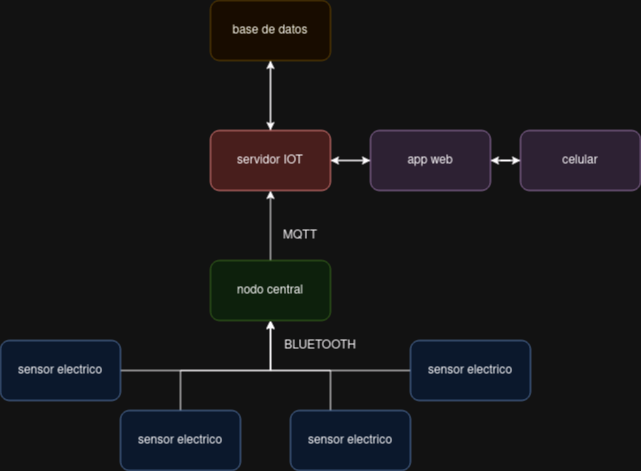
\includegraphics[width=.8\textwidth]{./Figuras/diagBloques.png}
\caption{Diagrama en bloques del sistema.}
\label{fig:diagBloques}
\end{figure}

\vspace{25px}

El usuario final, conectado desde un dispositivo móvil, podrá:

\begin{itemize}
\item{Verificar el consumo eléctrico de la red de dispositivos.
	}
\item{Configurar alarmas de exceso de consumo.
	}
\item{Verificar cortes en el consumo eléctrico.
	}
\item{Calcular el precio diferenciado por fecha y dispositivos.  
	}
\end{itemize}



\newpage

\section{2. Identificación y análisis de los interesados}
\label{sec:interesados}


En el cuadro \ref{tab:interesados} se presentan los interesados en el proyecto. 

\begin{table}[htbp]
\begin{tabularx}{\linewidth}{@{}|l|X|X|l|@{}}
\hline
\rowcolor[HTML]{C0C0C0} 
Rol           & Nombre y Apellido & Organización 	& Puesto 	\\ \hline
Auspiciante   & Ing. Martin Rodriguez                 &    Soft SA          	&       DBA 	\\ \hline
%Cliente       & \clientename      &\empclientename	&   Profesor FIUBA     	\\ \hline
Responsable   & \authorname       & FIUBA        	& Alumno 	\\ \hline
Colaboradores &   Sr. Gabriel Garcia                &              	&    Desempleado    	\\ \hline
Orientador    & \supname & \pertesupname 	& Director Trabajo final \\ \hline
Equipo        &  Ing. Guillermo Tala          			  &   Soft SA               		      &   Desarrollador  	\\ \hline
Usuario final &  Sra. Ana Alvarez                 &              	&       Jubilada 	\\ \hline
\end{tabularx}
\caption{Identificación de los interesados}
\label{tab:interesados}
\end{table}

\vspace{20px}

Se describen las características de los interesados en el proyecto:

\begin{itemize}
%	\item Auspiciante: esta dispuesto a gastar dinero para el proyecto.
%	\item Cliente: tiene experiencia previa en planificación, va a poder ayudar con la definición de los requerimientos y demás detalles. 
	\item Responsable: tiene la responsabilidad y el interes suficiente para terminar el proyecto.
	\item Colaboradores: esta desempleado y tiene el tiempo suficiente para comprar los materiales necesarios, va a poder ayudar mucho en cuestiones de logística.
	\item Orientador: es el especialista en esta tecnología.Se puede tener en cuenta  a la hora de evaluar alternativas.Cumple el rol de auspiciante y cliente ayudando en cuestiones economicas, como también en establecer requerimientos del proyecto.
	\item Equipo: Es especialista en desarrollo desde hace varios años. Planificar considerando que tiene poco tiempo extra laboral.
	\item Usuario Final: tiene la necesidad de probar el proyecto, por motivos económicos.
\end{itemize}




\section{3. Propósito del proyecto}
\label{sec:proposito}


El propósito de este proyecto es implementar un sistema IoT para monitorear el consumo eléctrico en viviendas y departamentos de un mismo predio.
Se pretende aplicar los conocimientos adquiridos para la gestión del proyecto y el diseño del sistema en todas sus etapas.


\section{4. Alcance del proyecto}
\label{sec:alcance}


El presente proyecto incluye:

\begin{itemize}
\item{Desarrollo de la aplicacion IoT( frontend, backend, base de datos ).}
\item{Desarrollo de firmware para módulos sensor y transmisor }
\item{Desarrollo de un prototipo  para el modulo sensor en protoboard o placa perforada}
\item{Desarrollo de un prototipo para el modulo transmisor ( interface sensores e internet ) en protoboard o placa perforada}
\end{itemize}




El presente proyecto no incluye:

\begin{itemize}
\item{La construcción y/o adaptación del PCB para los módulos sensor y transmisor.}
\item{La construcción y/o adaptación de un gabinete para los módulos sensor y transmisor.}
\item{El desarrollo de una aplicación de celular para sistemas Android o similares}
\end{itemize}




\section{5. Supuestos del proyecto}
\label{sec:supuestos}


Para el desarrollo del presente proyecto se supone que:

\begin{itemize}
\item{El modulo ESP32 tiene suficientes recursos para la implementación de este sistema.}
\item{Se conseguirán los materiales necesarios en el mercado local.}
\item{El diseño y desarrollo de código se realizará en tiempo y forma.}
\item{No se presentarán retrasos debidos a problemas de hardware, por ejemplo, en el diseño e implementación de los módulos sensor y transmisor.}
\item{El país no tendrá una devaluación lo suficientemente grande como para no poder contratar un servicio en la nube para alojar la aplicación.}
\end{itemize}







\section{6. Requerimientos}
\label{sec:requerimientos}

Se detallan los requerimientos necesarios dentro del proyecto:

\begin{enumerate}
	\item Requerimientos funcionales
		\begin{enumerate}
			\item El sistema debe ser capaz de medir el consumo eléctrico por hora, día , semana y mes.
			\item El modulo sensor y el modulo transmisor deben ser alimentados con la tension nominal de 220 Vac o en su defecto por una batería de 9 Vdc.
			\item El sistema debe ser capaz de monitorear el consumo del mismo dispositivo de medición.
			\item El dispositivo funcional debe poder trabajar en un rango de temperatura ambiente de 0°C a 50°C .
			\item El dispositivo funcional debe poder trabajar en un rango de corriente de 0 a 25 A .
			\item El dispositivo funcional debe poder trabajar a una frecuencia de 50 Hz.
			
		\end{enumerate}
		
	\item Requerimientos de documentación
		\begin{enumerate}
			\item La documentación debe contar con un esquemático de circuito eléctrico.
			\item La documentación debe contar con  un diagrama de la aplicación.
			\item La documentación debe contar con un manual de uso.
			\item La documentación debe contar con un manual de instalación.
		\end{enumerate}
		
	\item Requerimiento de testing
		\begin{enumerate}
			\item Se deben realizar pruebas de consumo eléctrico en un domicilio, con al menos dos dispositivos sensores por el periodo de una semana.
			\item Se deben contrastar las pruebas de consumo eléctrico con el medidor eléctrico del domicilio.
			\item Se debe controlar la correcta activación de las alarmas por exceso de consumo.
			\item Se debe controlar el correcto funcionamiento del dispositivo ante cortes en el suministro eléctrico.
								
		\end{enumerate}
	\item Requerimientos de la interfaz
		\begin{enumerate}
			\item El usuario debe poder configurar y visualizar alarmas por exceso de consumo eléctrico.
			\item El usuario debe poder seleccionar y visualizar el consumo eléctrico general por hora, día , semana y mes.
			\item El usuario debe poder seleccionar y visualizar el consumo eléctrico general promedio.
			\item El usuario debe poder seleccionar y visualizar el consumo eléctrico sensado por cada dispositivo.
			\item El usuario debe poder visualizar los cortes de suministro eléctrico.
			\item El usuario debe poder configurar alarmas por exceso de consumo eléctrico.	
			\item El usuario debe poder controlar el nivel de tension de batería auxiliar del dispositivo y notificar cuando la tension sea baja. 
		\end{enumerate}
	
	\item Requerimientos interoperabilidad
	\begin{enumerate}
		\item Los dispositivos sensores deben poder comunicarse via Bluetooth con el modulo transmisor.
		\item El modulo transmisor debe comunicarse con el servidor web por medio protocolo MQTT.
	\end{enumerate}
	
\end{enumerate}



\section{7. Historias de usuarios (\textit{Product backlog})}
\label{sec:backlog}

Las historias de usuario para el proyecto son las siguientes:

\begin{itemize}

\item{Como administrador  de un departamento necesito saber el consumo eléctrico mensual de cada domicilio para distribuir los gastos equitativamente sobre los inquilinos.}


Dificultad: media (3) → porque necesita mas dispositivos conectados en un mismo tablero.

Complejidad: baja (1) → Seria la misma implementación que para pocos dispositivos.

Riesgo: medio (3) → No tener el suficiente espacio para conectar todos los dispositivos en un mismo tablero eléctrico.

Story Point: 8 

(3 + 1 + 3 = 7 → 8 es el valor más cercano en Fibonacci)


\item{Como dueño de esta vivienda diariamente necesito saber  si estoy excediendo  el consumo eléctrico de una vivienda tipo, para no incurrir en multas o penalidades.
}

Dificultad: alta (5) → porque necesita saber los limites de consumo eléctrico de cada empresa para cada mes.

Complejidad: baja (1) → Se podría implementar un alerta automático para el cambio de los limites de consumo por mes. 

Riesgo: medio (3) → No poder actualizar obtener o estimar mensualmente los valores limites de consumo sin penalización. 

Story Point: 13 

(5 + 1 + 3 = 9 → 13 es el valor más cercano en Fibonacci)

\item{Como inquilino me gustaría saber el consumo eléctrico de los electrodomésticos de mi casa para evaluar el remplazo u otra alternativa.
}

Dificultad: media (3) → porque necesita mas dispositivos conectados.

Complejidad: baja (1) → Seria el mismo sistema con mas dispositivos conectados.

Riesgo: alta (5) → El electrodoméstico puede ser que consuma mucha potencia.

Story Point: 13 

(3 + 1 + 5 = 9 → 13 es el valor más cercano en Fibonacci)

\item{Como propietario deseo ver desde el celular los consumos eléctricos para no registrar un control manualmente desde el medidor.}


Dificultad: baja (1) → porque necesita un solo dispositivo conectado al tablero.

Complejidad: baja (1) → La implementación mas sencilla del sistema.

Riesgo: baja (1) → Solo requiere de la implementación de un solo dispositivo.

Story Point: 3 

(1 + 1 + 1 = 3 → 3 es el valor más cercano en Fibonacci)

\item{Como desarrollador deseo implementar la infraestructura de la aplicación en la nube para hacer mas escalable la aplicación.}


Dificultad: media (3) → porque se necesitan conocimientos técnicos para la implementación en la nube para no incurrir en gastos innecesarios.

Complejidad: alta (5) → Es un arquitectura relativamente compleja.

Riesgo: medio (3) → No disponer del tiempo y conocimiento suficiente para implementar la aplicación.

Story Point: 13 

(3 + 5 + 3 = 11 → 13 es el valor más cercano en Fibonacci)


\end{itemize}



\section{8. Entregables principales del proyecto}
\label{sec:entregables}


Los entregables del proyecto son :

\begin{itemize}
	
	\item Esquemáticos del circuito para el modulo sensor y modulo transmisor.
	\item Código fuente del firmware en codigo C, diseñado para la placa ESP32
	\item Diagrama de la aplicación	IoT
	\item Código fuente de la aplicación IoT
	\item Prototipo funcional verificado	
	\item Manual de instalación
	\item Manual de uso
	\item Informe final
	
\end{itemize}


\section{9. Desglose del trabajo en tareas}
\label{sec:wbs}

Las tareas a realizar son las siguientes:

\begin{enumerate}
\item Investigación inicial. (40 hs)
	\begin{enumerate}
	\item Investigación sobre proyectos existentes.	(8 hs)
	\item Investigación sobre el modulo sensor con conexión Bluetooth. (8 hs)
	\item Investigación sobre el modulo transmisor con conexión MQTT. (8 hs)
	\item Investigación sobre librerías existentes de la placa ESP32. (8 hs)
	\item Investigación sobre aplicaciones implementadas en la nube. (8 hs)
	\end{enumerate}
\item Materiales necesarios. (28 hs)
	\begin{enumerate}
	\item Identificar los proveedores para los materiales necesarios. (8 hs)
	\item Comprar los materiales.(6 hs)
	\item Identificar los proveedores de servicios en la nube. (8 hs)
	\item Contratar servicios en la nube. (6 hs)
	\end{enumerate}
\item Desarrollo de hardware. (76 hs)
	\begin{enumerate}
	\item Diseño de circuito esquemático en protoboard. (20 hs)
	\item Implementación en protoboard. (20 hs)
	\item Diseño de circuito en placa perforada. (10 hs)
	\item Implementación en placa perforada.(10 hs)
	\item Primer chequeo del funcionamiento de los modulos. (8 hs)
	\item Correcciones en el circuito. (8 hs)
	\end{enumerate}
\item Desarrollo de firmware. (68 hs)
	\begin{enumerate}
	\item Confección del diagrama de bloques del código. (8 hs)
	\item Desarrollo de código C para la comunicación UART(Bluetooth). (12 hs)
	\item Desarrollo de código C para la comunicación MQTT.	(12 hs)
	\item Desarrollo de código para consumo de batería.	(12 hs)
	\item Primer chequeo del funcionamiento del firmware.(8 hs)
	\item Correcciones en el funcionamiento del firmware.(16 hs)
	\end{enumerate}
\item Desarrollo de aplicación. (116 hs)
	\begin{enumerate}
	\item Confección de un diagrama de la aplicación IoT. (8 hs)
	\item Confección de un diagrama en bloques del código. (8 hs)
	\item Desarrollo de código frontend. (36 hs)
	\item Desarrollo de código backend. (36 hs)
	\item Integración de la aplicación en la nube. (12 hs)
	\item Primer chequeo del funcionamiento de la  aplicación. (8 hs)
	\item Correcciones en el funcionamiento de la  aplicación. (16 hs)
	\end{enumerate}

\item Etapa de integración. (32 hs)
	\begin{enumerate}
	\item Integración de software y  hardware. (16 hs)
	\item Correcciones generales de software y  hardware. (16 hs)
	\end{enumerate}
	
\item Testing del proyecto. (36 hs)
	\begin{enumerate}
	\item Instalación del sistema en un domicilio. (8 hs)
	\item Pruebas de consumo eléctrico en un domicilio.	(4 hs)
	\item Pruebas del dispositivo ante cortes de suministro eléctrico.	(4 hs)
	\item Pruebas del sistema de alarmas del dispositivo. (4 hs)
	\item Correcciones generales del sistema. (16 hs)
	\end{enumerate}
	
\item Verificación del prototipo. (8 hs)
	\begin{enumerate}
	\item Verificación de la interfaz de usuario. (8 hs)
	\end{enumerate}	
	
\item Documentación. (104 hs)
	\begin{enumerate}
	\item Documentación de esquemáticos.(8 hs)
	\item Documentación del código C. (16 hs)
	\item Documentación de la aplicación IoT. (16 hs)
	\item Documentación del manual de instalación. (16 hs)
	\item Documentación del manual de uso. (16 hs)
	\item Documentación del informe final. (32 hs)

	\end{enumerate}


\end{enumerate}

Cantidad total de horas: (508 hs)



\section{10. Diagrama de Activity On Node}
\label{sec:AoN}

\begin{consigna}{red}
Armar el AoN a partir del WBS definido en la etapa anterior. 

%La figura \ref{fig:AoN} fue elaborada con el paquete latex tikz y pueden consultar la siguiente referencia \textit{online}:

%\url{https://www.overleaf.com/learn/latex/LaTeX_Graphics_using_TikZ:_A_Tutorial_for_Beginners_(Part_3)\%E2\%80\%94Creating_Flowcharts}

\end{consigna}

\begin{figure}[htpb]
\centering 
\includegraphics[width=.8\textwidth]{./Figuras/AoN.png}
\caption{Diagrama de \textit{Activity on Node}.}
\label{fig:AoN}
\end{figure}

Indicar claramente en qué unidades están expresados los tiempos.
De ser necesario indicar los caminos semicríticos y analizar sus tiempos mediante un cuadro.
Es recomendable usar colores y un cuadro indicativo describiendo qué representa cada color, como se muestra en el siguiente ejemplo:



\section{11. Diagrama de Gantt}
\label{sec:gantt}

\begin{consigna}{red}

Existen muchos programas y recursos \textit{online} para hacer diagramas de Gantt, entre los cuales destacamos:

\begin{itemize}
\item Planner
\item GanttProject
\item Trello + \textit{plugins}. En el siguiente link hay un tutorial oficial: \\ \url{https://blog.trello.com/es/diagrama-de-gantt-de-un-proyecto}
\item Creately, herramienta online colaborativa. \\\url{https://creately.com/diagram/example/ieb3p3ml/LaTeX}
\item Se puede hacer en latex con el paquete \textit{pgfgantt}\\ \url{http://ctan.dcc.uchile.cl/graphics/pgf/contrib/pgfgantt/pgfgantt.pdf}
\end{itemize}

Pegar acá una captura de pantalla del diagrama de Gantt, cuidando que la letra sea suficientemente grande como para ser legible. 
Si el diagrama queda demasiado ancho, se puede pegar primero la ``tabla'' del Gantt y luego pegar la parte del diagrama de barras del diagrama de Gantt.

Configurar el software para que en la parte de la tabla muestre los códigos del EDT (WBS).\\
Configurar el software para que al lado de cada barra muestre el nombre de cada tarea.\\
Revisar que la fecha de finalización coincida con lo indicado en el Acta Constitutiva.

En la figura \ref{fig:gantt}, se muestra un ejemplo de diagrama de Gantt realizado con el paquete de \textit{pgfgantt}. En la plantilla pueden ver el código que lo genera y usarlo de base para construir el propio.

\begin{figure}[htbp]
\begin{center}
\begin{ganttchart}{1}{12}
  \gantttitle{2020}{12} \\
  \gantttitlelist{1,...,12}{1} \\
  \ganttgroup{Group 1}{1}{7} \\
  \ganttbar{Task 1}{1}{2} \\
  \ganttlinkedbar{Task 2}{3}{7} \ganttnewline
  \ganttmilestone{Milestone o hito}{7} \ganttnewline
  \ganttbar{Final Task}{8}{12}
  \ganttlink{elem2}{elem3}
  \ganttlink{elem3}{elem4}
\end{ganttchart}
\end{center}
\caption{Diagrama de Gantt de ejemplo}
\label{fig:gantt}
\end{figure}


\begin{landscape}
\begin{figure}[htpb]
\centering 
\includegraphics[height=.85\textheight]{./Figuras/Gantt-2.png}
\caption{Ejemplo de diagrama de Gantt rotado}
\label{fig:diagGantt}
\end{figure}

\end{landscape}

\end{consigna}


\section{12. Presupuesto detallado del proyecto}
\label{sec:presupuesto}

\begin{consigna}{red}
Si el proyecto es complejo entonces separarlo en partes:
\begin{itemize}
	\item Un total global, indicando el subtotal acumulado por cada una de las áreas.
	\item El desglose detallado del subtotal de cada una de las áreas.
\end{itemize}

IMPORTANTE: No olvidarse de considerar los COSTOS INDIRECTOS.

\end{consigna}

\begin{table}[htpb]
\centering
\begin{tabularx}{\linewidth}{@{}|X|c|r|r|@{}}
\hline
\rowcolor[HTML]{C0C0C0} 
\multicolumn{4}{|c|}{\cellcolor[HTML]{C0C0C0}COSTOS DIRECTOS} \\ \hline
\rowcolor[HTML]{C0C0C0} 
Descripción &
  \multicolumn{1}{c|}{\cellcolor[HTML]{C0C0C0}Cantidad} &
  \multicolumn{1}{c|}{\cellcolor[HTML]{C0C0C0}Valor unitario} &
  \multicolumn{1}{c|}{\cellcolor[HTML]{C0C0C0}Valor total} \\ \hline
 &
  \multicolumn{1}{c|}{} &
  \multicolumn{1}{c|}{} &
  \multicolumn{1}{c|}{} \\ \hline
 &
  \multicolumn{1}{c|}{} &
  \multicolumn{1}{c|}{} &
  \multicolumn{1}{c|}{} \\ \hline
\multicolumn{1}{|l|}{} &
   &
   &
   \\ \hline
\multicolumn{1}{|l|}{} &
   &
   &
   \\ \hline
\multicolumn{3}{|c|}{SUBTOTAL} &
  \multicolumn{1}{c|}{} \\ \hline
\rowcolor[HTML]{C0C0C0} 
\multicolumn{4}{|c|}{\cellcolor[HTML]{C0C0C0}COSTOS INDIRECTOS} \\ \hline
\rowcolor[HTML]{C0C0C0} 
Descripción &
  \multicolumn{1}{c|}{\cellcolor[HTML]{C0C0C0}Cantidad} &
  \multicolumn{1}{c|}{\cellcolor[HTML]{C0C0C0}Valor unitario} &
  \multicolumn{1}{c|}{\cellcolor[HTML]{C0C0C0}Valor total} \\ \hline
\multicolumn{1}{|l|}{} &
   &
   &
   \\ \hline
\multicolumn{1}{|l|}{} &
   &
   &
   \\ \hline
\multicolumn{1}{|l|}{} &
   &
   &
   \\ \hline
\multicolumn{3}{|c|}{SUBTOTAL} &
  \multicolumn{1}{c|}{} \\ \hline
\rowcolor[HTML]{C0C0C0}
\multicolumn{3}{|c|}{TOTAL} &
   \\ \hline
\end{tabularx}%
\end{table}


\section{13. Gestión de riesgos}
\label{sec:riesgos}

\begin{consigna}{red}
a) Identificación de los riesgos (al menos cinco) y estimación de sus consecuencias:
 
Riesgo 1: detallar el riesgo (riesgo es algo que si ocurre altera los planes previstos de forma negativa)
\begin{itemize}
	\item Severidad (S): mientras más severo, más alto es el número (usar números del 1 al 10).\\
	Justificar el motivo por el cual se asigna determinado número de severidad (S).
	\item Probabilidad de ocurrencia (O): mientras más probable, más alto es el número (usar del 1 al 10).\\
	Justificar el motivo por el cual se asigna determinado número de (O). 
\end{itemize}   

Riesgo 2:
\begin{itemize}
	\item Severidad (S): 
	\item Ocurrencia (O):
\end{itemize}

Riesgo 3:
\begin{itemize}
	\item Severidad (S): 
	\item Ocurrencia (O):
\end{itemize}


b) Tabla de gestión de riesgos:      (El RPN se calcula como RPN=SxO)

\begin{table}[htpb]
\centering
\begin{tabularx}{\linewidth}{@{}|X|c|c|c|c|c|c|@{}}
\hline
\rowcolor[HTML]{C0C0C0} 
Riesgo & S & O & RPN & S* & O* & RPN* \\ \hline
       &   &   &     &    &    &      \\ \hline
       &   &   &     &    &    &      \\ \hline
       &   &   &     &    &    &      \\ \hline
       &   &   &     &    &    &      \\ \hline
       &   &   &     &    &    &      \\ \hline
\end{tabularx}%
\end{table}

Criterio adoptado: 
Se tomarán medidas de mitigación en los riesgos cuyos números de RPN sean mayores a...

Nota: los valores marcados con (*) en la tabla corresponden luego de haber aplicado la mitigación.

c) Plan de mitigación de los riesgos que originalmente excedían el RPN máximo establecido:
 
Riesgo 1: plan de mitigación (si por el RPN fuera necesario elaborar un plan de mitigación).
  Nueva asignación de S y O, con su respectiva justificación:
  - Severidad (S): mientras más severo, más alto es el número (usar números del 1 al 10).
          Justificar el motivo por el cual se asigna determinado número de severidad (S).
  - Probabilidad de ocurrencia (O): mientras más probable, más alto es el número (usar del 1 al 10).
          Justificar el motivo por el cual se asigna determinado número de (O).

Riesgo 2: plan de mitigación (si por el RPN fuera necesario elaborar un plan de mitigación).
 
Riesgo 3: plan de mitigación (si por el RPN fuera necesario elaborar un plan de mitigación).

\end{consigna}


\section{14. Gestión de la calidad}
\label{sec:calidad}

\begin{consigna}{red}
Elija al menos diez requerientos que a su criterio sean los más importantes/críticos/que aportan más valor y para cada uno de ellos indique las acciones de verificación y validación que permitan asegurar su cumplimiento.

\begin{itemize} 
\item Req \#1: copiar acá el requerimiento.

\begin{itemize}
	\item Verificación para confirmar si se cumplió con lo requerido antes de mostrar el sistema al cliente. Detallar 
	\item Validación con el cliente para confirmar que está de acuerdo en que se cumplió con lo requerido. Detallar  
\end{itemize}

\end{itemize}

Tener en cuenta que en este contexto se pueden mencionar simulaciones, cálculos, revisión de hojas de datos, consulta con expertos, mediciones, etc.  Las acciones de verificación suelen considerar al entregable como ``caja blanca'', es decir se conoce en profundidad su funcionamiento interno.  En cambio, las acciones de validación suelen considerar al entregable como ``caja negra'', es decir, que no se conocen los detalles de su funcionamiento interno.

\end{consigna}

\section{15. Procesos de cierre}    
\label{sec:cierre}

\begin{consigna}{red}
Establecer las pautas de trabajo para realizar una reunión final de evaluación del proyecto, tal que contemple las siguientes actividades:

\begin{itemize}
	\item Pautas de trabajo que se seguirán para analizar si se respetó el Plan de Proyecto original:
	 - Indicar quién se ocupará de hacer esto y cuál será el procedimiento a aplicar. 
	\item Identificación de las técnicas y procedimientos útiles e inútiles que se emplearon, y los problemas que surgieron y cómo se solucionaron:
	 - Indicar quién se ocupará de hacer esto y cuál será el procedimiento para dejar registro.
	\item Indicar quién organizará el acto de agradecimiento a todos los interesados, y en especial al equipo de trabajo y colaboradores:
	  - Indicar esto y quién financiará los gastos correspondientes.
\end{itemize}

\end{consigna}


\end{document}
